\documentclass{beamer}
\usepackage[english]{babel}
\usepackage{graphicx}
\usepackage{times}
\usepackage{wrapfig}
\newcommand{\BibTeX}{{\sc Bib}\TeX}
\begin{document}
\title{De Morgan's Laws}   
\author{Author:Shefali Garg\\11678\\CSE} 
\date{\today} 

\frame{\titlepage} 

\frame{\frametitle{Table of contents}\tableofcontents} 


\section{Logic Gates}
\subsection{And Gate} 
\frame{\frametitle{And Gate} 
For any two given inputs A and B,output X is given as\\
X=AB
\begin{figure}[htp]
  \caption{AND gate}
  \centering
    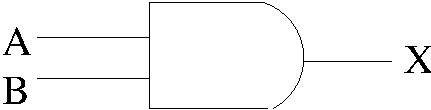
\includegraphics[width=0.2\textwidth]{AND}
\end{figure}
Truth table for AND gate \cite{and_gate97}
\newline
\newline
 \begin{tabular}{ | l | l | l |}
    \hline
    A & B & X \\ \hline
    1 & 1 & 1 \\ \hline
    1 & 0 & 0 \\ \hline
    0 & 1 & 0 \\ \hline
    0 & 0 & 0 \\ \hline
    \end{tabular}
   }
\subsection{Or Gate}
\frame{\frametitle{Or Gate} 
For any two given inputs A and B,output X is given as\\
X=A+B
\begin{figure}[htp]
  \caption{Or gate}
  \centering
    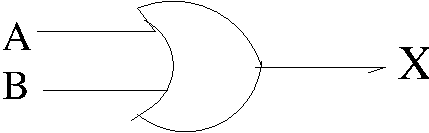
\includegraphics[width=0.2\textwidth]{OR}
\end{figure}
Truth table for Or gate \cite{or_gate93}
\newline
\newline
 \begin{tabular}{ | l | l | l |}
    \hline
    A & B & X \\ \hline
    1 & 1 & 1 \\ \hline
    1 & 0 & 1 \\ \hline
    0 & 1 & 1 \\ \hline
    0 & 0 & 0 \\ \hline
    \end{tabular}
   }
\subsection{Not Gate}
\frame{\frametitle{Not Gate} 
For given input A,output X is given as\\
X=$\overline{A}$
\begin{figure}[htp]
  \caption{Not gate}
  \centering
    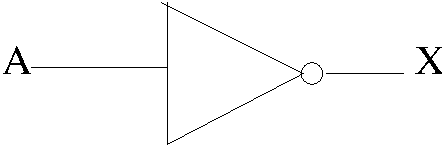
\includegraphics[width=0.2\textwidth]{not}
\end{figure}
Truth table for not gate \cite{not_gate97}
\newline
\newline
 \begin{tabular}{ | l | l |}
    \hline
    A & X \\ \hline
    1 & 0 \\ \hline
    0 & 1 \\ \hline
    \end{tabular}
   }
\section{De Morgan's laws}   
\frame{\frametitle{De morgan's laws for two variables} 
\begin{block}{}
Let A and B be two inputs.Then by De Morgan's laws \cite{morgan1999},
\begin{itemize}
\item $\overline{A+B}$ =$\overline{A}$  $\overline{B}$
\item $\overline{AB}=\overline{A}+\overline{B}$
\end{itemize}
\end{block}
}

\section{Prove De Morgan's Laws}
\subsection{First Law} 
\frame{\frametitle{Prove of First Law} 
According to first law,an OR gate with all inputs inverted (a Negative-OR gate) behaves the same as a NAND gate\\
that is, $\overline{AB}=\overline{A}+\overline{B}$
\begin{figure}[htp]
  \caption{First Law}
  \centering
    \includegraphics[width=0.2\textwidth]{law1}
\end{figure}
This can be proved by truth table
\newline
\newline
 \begin{tabular}{ | l | l | l | l | l | l | }
    \hline
    A & B & $\overline{AB}$ & $\overline{A}$ & $\overline{B}$ &$\overline{A}+\overline{B}$   \\ \hline
    1 & 1 & 0 & 0 & 0 & 0 \\ \hline
    1 & 0 & 1 & 0 & 1 & 1\\ \hline
    0 & 1 & 1 & 1 & 0 & 1 \\ \hline
    0 & 0 & 1 & 1 & 1 & 1 \\ \hline
    \end{tabular}
   }
 \subsection{Second Law} 
\frame{\frametitle{Proof of Second Law} 
According to first law,an AND gate with all inputs inverted (a Negative-AND gate) behaves the same as a NOR gate\\
that is, $\overline{A+B}$=$\overline{A}$  $\overline{B}$
\begin{figure}[htp]
  \caption{Second Law}
  \centering
    \includegraphics[width=0.2\textwidth]{law2}
\end{figure}
This can be proved by truth table
\newline
\newline
 \begin{tabular}{ | l | l | l | l | l | l | }
    \hline
    A & B & $\overline{A+B}$ & $\overline{A}$ & $\overline{B}$ &$\overline{A}$  $\overline{B}$   \\ \hline
    1 & 1 & 0 & 0 & 0 & 0 \\ \hline
    1 & 0 & 0 & 0 & 1 & 0\\ \hline
    0 & 1 & 0 & 1 & 0 & 0 \\ \hline
    0 & 0 & 1 & 1 & 1 & 1 \\ \hline
    \end{tabular}
   }  
\frame{\frametitle{De morgan's laws for n variables} 
\section{Generalised De Morgan's laws}   
\begin{block}{}
Let $x_1,x_2,...,x_n$ be two inputs.Then,
\begin{itemize}
\item $\overline{x_1+x_2+..+x_n} =\overline{x_1}\overline{x_2}...\overline{x_n}$
\item $\overline{x_1x_2...x_n}=\overline{x_1}+\overline{x_2}+...+\overline{x_n}$
\end{itemize}
\end{block}
}
\frame{\frametitle{References} 
\section{References}   
\bibliographystyle{plain}
\bibliography{gate}
}
   \end{document}